\documentclass{TIC_FC_EPN}    

\begin{document}
    
    \titulotic{Methods of time series data mining\\\vspace{0.3cm} Correlaciones entre espectros de series temporales magnéticas del método Empirical Mode Decomposition para datos de la Tierra y el Sol}

    \profesion{Físico}
    \estudiante{Luis Fernando Palacios Flores}
    \correoestudiante{luis.palacios01@epn.edu.ec}
    \director{Ramón Xulvi Brunet}
    \correodirector{ramon.xulvi@epn.edu.ec}
    \fecha{DMQ, Septiembre 2022}
    
    % Portada y documentos iniciales
    \portada
    \pagenumbering{roman}
    \setcounter{page}{1}
    \certificaciones
    \declaracionautoria
    
        \begin{dedicatoria}
    %     Inserte palabras bonitas.
    A toda alma insatisfecha que no detiene su movimiento.

\begin{flushright}
    \begin{spacing}{1.15}
        \textit{`` \hspace*{4cm} ... \hspace*{4cm} \\
                If you can meet with Triumph and Disaster\\
                And treat those two impostors just the same;\\
                \hspace*{4cm} ... \hspace*{4cm} \\
                Yours is the Earth and everything that’s in it,\\
            And—which is more—you’ll be a Man, my son!''
        }
    \end{spacing}
    - Rudyard Kipling, If    
\end{flushright}
    \end{dedicatoria}
    \begin{agradecimiento}
        A toda mi familiar, por todo su cariño y por creer en mí. En especial a mi padre, porque sin todo su apoyo, yo ya no estaría aquí.

        A los amigos que pude hacer en este breve momento de mi vida, entre ellos: Georgie, Daniel, André, Jorge, Cristopher, Valeria, Vladimir, Camila. Sin ellos la universidad no hubiera sido lo mismo. 
        
        Al mi tutor, el Dr. Ramón Xulvi, por todo el tiempo dedicado a la realización de este trabajo. Agradezco también por aportar más que solo conocimiento sino también por darme la oportunidad de pensar de manera diferente y continuar con mi crecimiento tanto académico como personal.  
        
        Al Dr. Luca Sorriso-Valvo por su colaboración en el desarrollo de este trabajo.  
        
        En sí, a todos los que a lo largo de mi periodo en la universidad me acompañaron, apoyaron y me permitieron crecer tanto en lo académico como en lo personal.
        
    \end{agradecimiento}
    
    \tableofcontents
    \addcontentsline{toc}{section}{\textbf{ÍNDICE GENERAL}}
    \begin{spacing}{1.22}
        \listoffigures % En caso de no tener figuras, comentar esta línea
    \end{spacing}    
    \addcontentsline{toc}{section}{\textbf{ÍNDICE DE FIGURAS}}

    \newpage
    
        \begin{resumen}
                    
        El viento solar es un plasma turbulento que lleva el campo magnético del Sol a medida que se expande a través del espacio interplanetario. En este trabajo se estudian las correlaciones entre las mediciones de las sondas espaciales Parker Solar Probe y Solar Orbiter, en el seguimiento de una parcela de plasma a medida que evoluciona radialmente desde el Sol hasta los alrededores de la Tierra. El método Empirical Mode Decomposition se usa para filtrar las altas frecuencias y reducir la influencia de la turbulencia. Los resultados sugieren que las series temporales pueden ser reconstruidas con la mitad de las componentes oscilatorias de menor frecuencia y conservar su comportamiento, realizando un buen filtrado de las altas frecuencias y obteniendo valores significativos en el cálculo de su correlación. Además, se observó la existencia de pares de intervalos de tiempo, en las series temporales, cuya correlación es alta, y que están relacionados con los datos del mismo plasma.  
        
    \vspace{0.3cm}\noindent\textbf{\textit{Palabras clave:}} Viento solar, turbulencia, altas frecuencias, función cross-correlation, método Empirical Mode Decomposition. 
    
    \end{resumen}
    
    \begin{resumenEng}
    
        The solar wind is a turbulent plasma that carries the Sun's magnetic field as it expands through interplanetary space. Here, correlations between the measurements of the Parker Solar Probe and Solar Orbiter spacecrafts are studied, in the tracking of a plasma parcel as it evolves radially from the Sun to the surroundings of the Earth. The Empirical Mode Decomposition method is used to filter out high frequencies and reduce the influence of turbulence. Results suggest that time series can be reconstructed with half of the lower frequency oscillatory components and preserve their behavior, performing a good filtering of high frequencies and obtaining significant values in the calculation of their correlation. Furthermore, it was observed the existence of pairs of time intervals, in the time series, whose correlation is high, and which are related to data of the same plasma.
        
    \vspace{0.3cm}\noindent\textbf{\textit{Keywords:}} Solar wind, turbulence, high frequencies, cross-correlation function, Empirical Mode Decomposition method.  
    \end{resumenEng}
         
     % Contenido
    \pagenumbering{arabic}
     \setcounter{page}{1}
     \chapter{Descripción del componente desarrollado}

\section{Marco teórico}

\subsection{Definición de un plasma}

\noindent Un plasma consiste en una colección de partículas cargadas (iones y electrones), además de átomos y moléculas neutras en ciertos casos \cite{Umran, Chen, Parks}. La formación de un plasma se produce cuando aumenta la temperatura de un gas neutro, o cuando se somete a campos eléctricos muy grandes, hasta que sus átomos y moléculas se ionizan \cite{Umran, Chen}. Por lo anterior, un plasma también puede considerarse como un gas ionizado. Por otro lado, la naturaleza cargada de las partículas de un plasma hace que sus propiedades sean diferentes a un gas normal, un líquido o un sólido, razón por la que se conoce como el cuarto estado de la materia \cite{Umran}. Es más, la mayoría de la materia ordinaria del universo se encuentra en estado de plasma \cite{Chen}.

% Un plasma tiene ciertas características fundamentales que lo diferencian de un gas ionizado. Las partículas cargadas de un plasma tienden a apantallar los campos eléctricos creados por cualquier perturbación eléctrica dentro de una distancia mucho menor que la dimensión característica del plasma \cite{Umran, Chen, Parks}. La distancia a la que sucede este apantallamiento se conoce como longitud de Debye. A distancias mayores que la longitud de Debye las interacciones individuales entre las partículas cargadas dejan de ser dominantes y el plasma tiene un comportamiento “colectivo” \cite{Kamide}. Esto quiere decir que el movimiento de las partículas no depende de las condiciones locales sino del plasma en su totalidad. Además, debido al apantallamiento las cargas se reorganizan de tal manera que en un plasma la densidad de iones positivos es aproximadamente igual a la densidad de electrones, y se dice que un plasma es un gas cuasi neutral \cite{Parks, Umran}. Esta tendencia a mantener la neutralidad provoca que los electrones de un plasma oscilen a una frecuencia característica en la que ocurren las perturbaciones electrostáticas en los plasmas.  Esta frecuencia de oscilación de electrones es mayor que la frecuencia a la que colisionan las partículas en el plasma, pues de lo contrario se pierde el comportamiento colectivo \cite{Chen}.


\subsection{Descripciones de un plasma}

\noindent En física de plasmas existen varios modelos para describir a un plasma. Dependiendo de las condiciones supuestas y de las diferentes aproximaciones que se realicen, un plasma se puede estudiar a través del movimiento de partículas individuales sujetas a la fuerza de Lorentz, mediante funciones de distribución a partir de la ecuación de Boltzmann debido al gran número de partículas presentes en el plasma, o por medio de las ecuaciones de la mecánica de fluidos, en conjunto con las ecuaciones del electromagnetismo, enfocándose en las propiedades colectivas del plasma \cite{Umran, Chen, Krall}.   

El enfoque fluido es muy importante al proporcionar una descripción \textit{macroscópica} de un plasma. Esta descripción es útil por las propiedades comunes entre un plasma y un fluido conductor, mostrando movimientos colectivos como, por ejemplo, ondas \cite{Krall}. En este modelo se considera a todo el plasma como un fluido de un solo tipo, enfocándose en las propiedades colectivas y despreciando la diferencia entre las partículas cargadas \cite{Umran, Chen}. Este enfoque se conoce como magnetohidrodinámica y es muy útil para describir un amplio rango de comportamientos de un plasma, abarcando la física espacial y de fusión \cite{Umran}. 

\subsection{El Sol y el Viento Solar}

\noindent El Sol es la principal fuente de energía que mantiene la vida en el planeta Tierra.  Es un plasma conformado con alrededor de $90\%$ de hidrógeno, $10\%$ de helio y una pequeña proporción de otros elementos tales como carbono, nitrógeno, y oxígeno \cite{Parks}. La temperatura en su interior ronda los $15 \times 10^{6} K$, permitiéndole producir energía a través de la fusión nuclear de hidrógeno en helio \cite{Cravens}. Una pequeña proporción de la energía generada viaja alrededor de $1.496 \times 10^{8} km$ para llegar desde el Sol hasta la Tierra \cite{Kamide}. Esta distancia define la unidad astronómica (UA).

La atmósfera del Sol se encuentra dividida en la fotosfera, la cromosfera, y la corona \cite{Parks, Cravens}. Esta última capa se sitúa sobre la otras dos y se extiende hacia el espacio interplanetario \cite{Kamide}. La expansión de la corona produce un flujo de partículas cargadas que son expulsadas por el Sol, comúnmente conocido como viento solar, y se descubrió en los comienzos de la era espacial \cite{Parks}. El viento solar es una consecuencia natural de estrellas calientes como el Sol, pues cuando la temperatura de la corona es de alrededor de $10^6 K$, casi el $50\%$ de los electrones tienen velocidades térmicas que exceden la velocidad de escape gravitacional del Sol, aunque en el caso de los protones es de menos del $1\%$ \cite{Parks, encrenaz_solar_2004}, debido a su mayor masa. Sin embargo, el exceso de carga positiva se contrarresta por la generación de un enorme campo eléctrico que provoca la aceleración de protones, expulsándolos del Sol \cite{encrenaz_solar_2004}. Por tanto, la expansión de la corona es una manera en la que el Sol mantiene su neutralidad de carga \cite{Parks}. 

El Sol tiene un campo magnético que a grandes escalas se aproxima a un dipolo magnético \cite{Cravens}, cuya intensidad superficial promedio es de alrededor de $10^{-4} T$ \cite{Parks, Kamide, Cravens}. En su expansión a través del espacio interplanetario, el viento solar lleva consigo el campo magnético del Sol que se extiende radialmente hacia afuera \cite{Kamide} y cubre todo el sistema solar, protegiendo a los planetas de las partículas de alta energía del espacio interestelar. El límite en donde se encuentra el viento solar con el viento interestelar se llama heliopausa, mientras que la región en su interior se denomina heliosfera \cite{Parks, encrenaz_solar_2004}, debido a la mayor influencia del Sol. Mediciones realizadas por magnetómetros en sondas espaciales muestran que la intensidad de campo magnético interplanetario alrededor de la Tierra es de unos pocos $10^{-9} T$ \cite{Parks, Kamide}. 

\subsection{Misiones de Exploración Espacial y Series Temporales}

\noindent Las sondas espaciales permiten mejorar la comprensión del espacio a través de la recopilación de información de gran interés científico. Los instrumentos a bordo son capaces de realizar mediciones y observaciones que en la Tierra no serían posibles. En particular, las misiones Parker Solar Probe (PSP), a cargo de la NASA y lanzada en 2018 \cite{fox_solar_2016}, y Solar Orbiter (SolO), dirigida por la ESA y lanzada en 2020 \cite{muller_solar_2020}, están encargadas de estudiar la heliosfera interior, enfocándose en el Sol. Estas sondas espaciales llevan instrumentos de detección a distancia (por ejemplo, telescopios) e in-situ (por ejemplo, magnetómetros), para realizar observaciones de la corona solar y para medir el viento solar, las partículas energéticas y los campos electromagnéticos \cite{fox_solar_2016, muller_solar_2020}, respectivamente. En conjunto, las sondas PSP y SolO posibilitan profundizar el entendimiento sobre la atmósfera del Sol y su actividad \cite{velli_understanding_2020}. 
    
Los instrumentos de las sondas espaciales registran los valores de diferentes magnitudes físicas a intervalos de tiempo iguales. A este tipo de mediciones se les conoce como series temporales \cite{Priestley, chatfield_analysis_2019}. De las series temporales registradas por las sondas espaciales son de especial interés las mediciones del campo magnético. 

La dinámica de los plasmas espaciales es un proceso intrínsecamente no lineal \cite{Kamide, bruno_turbulence_2016, matthaeus_intermittency_2015} y en general, no estacionario \cite{chatfield_analysis_2019, Priestley, alberti_multifractal_2019}. Esto último significa que las propiedades estadísticas (por ejemplo, la media y la varianza) de las series temporales cambian con el tiempo \cite{chatfield_analysis_2019, Priestley} y, por consiguiente, los datos no son estacionarios. Por otro lado, se dice que un sistema lineal tiene ``datos lineales”.          

\subsection{Turbulencia}

\noindent El movimiento de los fluidos se puede dividir en dos tipos, laminares o turbulentos. El primer caso implica un movimiento regular y suave del fluido, es decir, un movimiento ``predecible'' \cite{Landau, Cengel, davidson_turbulence_2015}. Por otro lado, un flujo turbulento se caracteriza por tener un carácter aleatorio e impredecible \cite{Landau, Cengel, davidson_turbulence_2015}. Por ejemplo, el flujo de humo de un cigarro que se deja consumir es laminar al principio, pero a medida que el humo se desplaza se vuelve turbulento formando remolinos de diversos tamaños que se mueven aleatoriamente \cite{Cengel}. 

La turbulencia es un fenómeno que se puede manifestar en cualquier fluido, pues el movimiento de un fluido es casi siempre inestable \cite{davidson_turbulence_2015}. No existe una definición rigurosa sobre la turbulencia, pero se distinguen características que permiten cierto entendimiento. El carácter impredecible de la turbulencia se debe a la sensibilidad a las condiciones iniciales, lo cual refleja su naturaleza caótica \cite{davidson_turbulence_2015}. De igual manera, grandes fluctuaciones en la velocidad del fluido son propias de la turbulencia \cite{davidson_turbulence_2015, Cengel}. Además, es común la presencia de remolinos que se forman y desplazan de manera aleatoria, como se mencionó en el ejemplo anterior. Finalmente, en un flujo turbulento, como resultado de la difusión del fluido, se produce disipación de energía, desde remolinos grandes hacia remolinos cada vez más pequeños, en la denominada cascada de energía de Richardson \cite{davidson_turbulence_2015, bruno_turbulence_2016}. 

\subsubsection{Turbulencia en el Viento Solar}

\noindent Los plasmas espaciales y los fluidos atmosféricos son sistemas turbulentos en evolución dinámica, cuyas interacciones son no lineales \cite{Kamide}. La naturaleza de las interacciones en estos sistemas es evidente cuando se tiene presente que algunas de las ecuaciones de la mecánica de fluidos son ecuaciones diferenciales no lineales parciales acopladas. En el caso del viento solar, las mediciones realizadas por sondas espaciales han demostrado que la turbulencia es un fenómeno que muestra la presencia de fluctuaciones a pequeña escala (espaciales y temporales) en el campo magnético, el campo de velocidades y la densidad de protones \cite{bruno_turbulence_2016, sorriso-valvo_intermittency_1999, hnat_intermittency_2003}. En el viento solar, la turbulencia se desarrolla fuertemente durante el desplazamiento y expansión a través del espacio interplanetario \cite{coleman_turbulence_1968, bruno_solar_2013, bruno_turbulence_2016}, similar al ejemplo del humo de cigarro.

\section{Motivación}

\noindent El alineamiento de sondas espaciales es un evento poco común del cual solamente se tienen unos pocos casos registrados \cite{damicis_radial_2010, bruno_spectral_2014, bruno_radial_2014, schwartz_radial_1983, zank_theory_2017, telloni_evolution_2021} desde que se empezaron a realizar mediciones in situ de la actividad magnética del Sol hace unas pocas décadas. Estos sucesos son de gran importancia para la investigación de las características de los plasmas espaciales porque permiten estudiar la evolución del plasma a través de la heliosfera.

En particular, el seguimiento de un plasma espacial permite estudiar las propiedades de la turbulencia del viento solar, lo cual es crucial para el entendimiento de los plasmas y en general, de los fluidos. Esto se realiza analizando la influencia de la turbulencia sobre las variables que se registran en series temporales. Recientemente, las sondas Parker Solar Probe y Solar Orbiter, tuvieron su primer alineamiento radial a una distancia de $ \sim 0.1 UA$ y $ \sim 1 UA$ \cite{telloni_evolution_2021}, respectivamente. Las mediciones del campo magnético del viento solar mostraron que el plasma pasa de un estado poco turbulento cerca del Sol hacia un comportamiento con una turbulencia altamente desarrollada e intermitente en las cercanías de la Tierra \cite{telloni_evolution_2021}. La motivación detrás de este trabajo es investigar la evolución de la parte no turbulenta del campo magnético cuando el viento solar se desplaza radialmente desde el Sol hasta la Tierra. Esta parte no turbulenta se puede cuantificar mediante un filtrado de las altas frecuencias de las series temporales asociadas.

El tipo de análisis que se realiza sobre las series temporales es crucial en cuanto a las características que se pretenden estudiar. La correlación es una medida estadística de uso frecuente para analizar series temporales. Esta mide el grado de similitud entre dos series temporales \cite{chatfield_analysis_2019}. Por ejemplo, en el seguimiento de un plasma espacial, las series temporales de cada sonda deben estar altamente correlacionadas para concluir que pertenecen al mismo plasma.

Es común que el análisis de las series temporales de los plasmas espaciales se realice mediante métodos estándar como aquellos basados en la transformada de Fourier o transformadas wavelet \cite{chatfield_analysis_2019}. Sin embargo, los primeros solamente son útiles para datos estacionarios \cite{chatfield_analysis_2019}, mientras que los últimos están restringidos a datos con escalas temporales definidas \cite{huang_empirical_1998, Percival}. Además, algunos de los métodos estándar son estrictamente útiles para datos que provienen de sistemas lineales, o son muy especializados para explorar nuevas características en los datos. Por otro lado, las series temporales de las magnitudes físicas del viento solar son no lineales, no estacionarias y dependen de la escala \cite{de_michelis_multi-scale_2012, carbone_arbitrary-order_2018, alberti_multifractal_2019, carbone_statistical_2020, carbone_statistical_2021}, es decir, de los intervalos espaciales y temporales en donde ocurren ciertos procesos físicos.   

El método Empirical Mode Decomposition (EMD) puede ser útil para el análisis de series temporales magnéticas \cite{de_michelis_multi-scale_2012, carbone_arbitrary-order_2018, alberti_multifractal_2019, carbone_statistical_2020, carbone_statistical_2021}. Este método descompone una serie temporal en una suma de componentes oscilatorias denominadas funciones de modo intrínseco (IMFs), que permiten una buena reconstrucción de la serie. Reconstrucciones parciales (no todas las IMFs) hacen posible filtrar las componentes de alta frecuencia de las series temporales. Debido al carácter empírico del método, las características locales de la escala de tiempo de los datos son consideradas \cite{huang_empirical_1998}, y esto hace posible estudiar un mayor tipo de datos. Por esta razón, en este trabajo se utiliza el EMD para analizar las series temporales del viento solar durante el alineamiento de las sondas espaciales PSP y SolO. 

\section{Objetivos}

\subsection{Objetivo General}

\noindent En este estudio se busca identificar posibles correlaciones relevantes entre las reconstrucciones a baja frecuencia de las series temporales de campo magnético del viento solar, en los alrededores del Sol y la Tierra (medidas por PSP y SolO, respectivamente), obtenidas mediante las IMFs de la descomposición del método Empirical Mode Decomposition. De esta manera se quiere estimar si se puede disminuir la aparente aleatoriedad que aporta la turbulencia sobre las series temporales y conservar resultados significativos.

%Para cumplir el objetivo general de este trabajo se plantean los siguientes objetivos específicos:

\subsection{Objetivos Específicos}

\begin{enumerate}
    \item Implementar y aplicar el método Empirical Mode Decomposition a las series temporales.
    \item Implementar el método Cross-Correlation y aplicarlo entre reconstrucciones de las series temporales realizadas a partir de sus IMFs de menor frecuencia.  
\end{enumerate}

\section{Alcance}

\noindent El presente trabajo pretende ser un estudio exploratorio de la evolución de la parte no turbulenta de las series temporales del campo magnético al filtrar las componentes de alta frecuencia mediante el EMD. Además, se indaga en el número de IMFs necesario para reconstruir las series temporales y obtener resultados significativos en el cálculo de las correlaciones entre las series.

En este trabajo se utilizaron datos que derivan de otro estudio de series temporales de campo magnético, que también corresponden con el alineamiento de las sondas espaciales PSP y SolO \cite{telloni_evolution_2021}. Los datos recibidos fueron preprocesados por el grupo de investigación anterior por lo que se pudo omitir este paso en el análisis de las series temporales. Esto permitió continuar con la implementación y aplicación del método EMD, que en este caso se realizó en Fortran. También se utilizaron las librerías de Matlab y Python para comparar y validar la implementación realizada. 

El método Cross-Correlation es uno de los métodos estándar más utilizados para correlacionar series temporales \cite{chatfield_analysis_2019}. Este método se implementó en Python debido a la eficiencia de tiempo, manejo y almacenamiento de variables, para el caso particular del cálculo de las correlaciones propuestas. 
     \chapter{Metodología}

\section{Descripción de los datos}

\noindent Las series temporales de campo magnético del viento solar provienen de mediciones in situ realizadas por las sondas espaciales PSP y SolO durante su primer alineamiento radial a una distancia de $ \sim 0.1 UA$ y $ \sim 1 UA$, respectivamente. Los datos de la sonda PSP fueron registrados el 27 de septiembre de 2020 desde las 03:05 UT hasta las 05:15 UT (130 minutos), y los datos de la sonda SolO fueron tomados el 01 de octubre de 2020 a las 21:20 UT hasta el 02 de octubre de 2020 a las 01:20 UT (240 minutos). La frecuencia de muestreo de los datos estudiados es de 8 $Hz$.  

\begin{figure}[H]
    \centering
    \includegraphics[scale=0.45]{data_PSP.png}
    \caption{Datos del campo magnético en la sonda PSP durante el intervalo de tiempo 03:05 - 05:15 UT el 27 de septiembre de 2020. De arriba hacia abajo: $B_{R}$ y $|B|$, $B_{T}$ y $B_{N}$.}
    \label{fig1}
\end{figure}

En las figuras \ref{fig1} y \ref{fig2} se muestra la intensidad de campo magnético ($|B|$) y sus componentes en el sistema de coordenadas RTN, para las series temporales de ambas sondas espaciales. En el sistema de coordenadas RTN, la componente R apunta radialmente desde el centro del Sol hasta la nave espacial; la componente tangencial T es el producto cruz de la velocidad angular del Sol con R; y la componente normal N completa la triada ortogonal y tiene la misma dirección que la velocidad angular del Sol \cite{bruno_turbulence_2016}.

\begin{figure}[H]
    \centering
    \includegraphics[scale=0.45]{data_SolO.png}
    \caption{Datos del campo magnético en la sonda SolO desde el 01 de octubre de 2020 a las 21:20 UT hasta el 02 de octubre de 2020 a las 01:20 UT. De arriba hacia abajo: $B_{R}$ y $|B|$, $B_{T}$ y $B_{N}$.}
    \label{fig2}
\end{figure}

\section{Empirical Mode Decomposition}\label{EMD}

\noindent Muchos de los fenómenos físicos en la naturaleza se caracterizan por tener una dinámica no lineal \cite{strogatz_nonlinear_2015} y, en muchas ocasiones, no estacionaria. Incluso el ejemplo más sencillo que se le puede ocurrir a un físico, como es el movimiento de un péndulo simple en ausencia de fuerzas externas y rozamiento es, en general, no lineal. Además, aún en el caso de pequeñas oscilaciones, cuando se considera un movimiento amortiguado, se pierde la estacionariedad, pues la amplitud de oscilación deja de ser constante y su valor medio cambia con el tiempo \cite{Priestley, chatfield_analysis_2019}.        

Los datos de series temporales pueden mostrar diversos patrones que son más fáciles de entender cuando se descomponen en varios componentes. Es como observar un reloj y tener una idea de cómo funciona, pero solamente entenderlo (o mejorar la comprensión) cuando se lo desarma y observa la posición de sus partes y cómo estas interactúan entre sí. De igual manera, descomponer una señal puede hacer más fácil su análisis cuando se hace uso de las técnicas adecuadas. Por ejemplo, la transformada de Fourier permite identificar las componentes de frecuencia de una señal y, operando sobre estas, filtrar las frecuencias \cite{rao_fast_2010} que no sean de interés.   

Los métodos estándar basados en la transformada de Fourier y la transformada Wavelet son muy utilizados para analizar series temporales pues están basados en una teoría matemática robusta \cite{huang_empirical_1998, Percival}, lo que facilita la interpretación de los resultados. Sin embargo, las teorías analíticas que soportan estos métodos requieren de propiedades de ortogonalidad y/o completitud, lo que fija a priori el número de componentes en las que se descompone una señal. Más aún, estas componentes pueden tener otras restricciones adicionales como ser funciones sinusoidales, el cual es el caso en la transformada de Fourier con los modos de oscilación armónicos. 

En una serie temporal cualquiera puede que su descomposición no sea idónea en componentes sinusoidales. Tampoco puede que exista un número fijo para el cual se obtenga una clara distinción entre ellas. Este es el caso de las series temporales que provienen de sistemas físicos no lineales, no estacionarios y que pueden tener diferentes escalas características. Por esta razón, el análisis y la descripción de estos sistemas requiere el uso de diferentes métodos basados en técnicas adaptativas que permitan describir sus características inherentes a partir de una descomposición basada en los propios datos.

El método Empirical Mode Decomposition (EMD) es un método adaptativo que se basa en la escala de tiempo característica local de los datos, permitiendo descomponer señales de procesos no lineales y no estacionarios \cite{huang_empirical_1998}. Es decir, este método analiza las características de los datos de punto a punto para realizar la descomposición sin importar si los procesos son no lineales o no estacionarios. Además, como el método está basado en los datos, la base de la descomposición se define a posteriori y no se imponen restricciones sobre estas componentes (amplitud constante y frecuencia fija en el caso de la expansión de Fourier). El EMD permite descomponer una señal en un número finito de componentes oscilatorias denominadas funciones de modo intrínseco (Intrinsic Mode Functions, IMFs), las cuales poseen amplitud y frecuencia moduladas. 

La descomposición de una serie temporal en sus IMFs se realiza mediante un proceso iterativo denominado \textit{sifting} (tamizado). El razonamiento detrás de este proceso consiste en extraer los componentes de una señal comenzando con aquellas de mayor frecuencia y con cada iteración separar los diferentes modos de una señal según sus características para de esta manera terminar con la IMF con menor frecuencia. Esto es similar a tener un arreglo de tamices diferentes. Al finalizar este proceso la serie temporal original $x(t)$ puede escribirse como la suma de $M$ modos oscilantes $c_{j}(t)$ (IMFs) y un residuo monótono $r(t)$, que representa la tendencia a largo plazo de la señal original, lo cual es usual en el análisis de series temporales \cite{chatfield_analysis_2019}. 

\begin{equation}
    x(t) = \sum_{j=1}^{M} c_{j}(t) + r(t)
    \label{emd}
\end{equation}

\newpage

Las IMFs que se obtienen tras la descomposición poseen dos propiedades importantes.

\begin{enumerate}[label=(\arabic*)]
    \hypertarget{imfs_cond1}{\item} El número de extremos y cruces por cero es igual o difieren como máximo en uno. 
    \hypertarget{imfs_cond2}{\item} El valor medio es cero. 
\end{enumerate}

La primera condición garantiza que no existan oscilaciones complicadas en las componentes de la descomposición y que exista un cruce por cero al menos una vez antes de que pasar de un extremo a otro, lo que dota a las IMFs de simetría y hace que el método sea adaptativo. Por otro lado, la segunda condición permite obtener frecuencias instantáneas que no sean afectadas por fluctuaciones asimétricas. Esto también implica que las IMFs son estacionarias (lo cual permite ampliar el análisis de las series temporales \cite{huang_amplitude-frequency_2008}). De esta manera, cada IMF tiene una amplitud modulada y frecuencias instantáneas físicamente significativas que pueden ser de banda estrecha \cite{huang_empirical_1998}.  

El proceso \textit{sifting} es la base del método EMD y los pasos que se utilizaron en este trabajo pueden resumirse en el siguiente algoritmo:    

\begin{spacing}{1}
    \begin{enumerate}[label=\arabic*.]
        \item Establecer la condición inicial para el residuo $r(t) = x(t)$.
        \item Identificar los máximos y mínimos locales de $x(t)$. 
        \item Usar la interpolación cubic splines para calcular las envolventes, superior $e_{max}(t)$ e inferior $e_{min}(t)$, definidas por los máximos y mínimos locales, respectivamente.  
        \item Calcular la envolvente media $e_{m}(t) = \frac{1}{2}(e_{min}(t) + e_{max}(t))$.
        \item Evaluar $h_{i}(t) = x(t) - e_{m}(t)$, denominada proto-IMF, y verificar si cumple con las condiciones \hyperlink{imfs_cond1}{(1)} y \hyperlink{imfs_cond2}{(2)} para ser una IMF.
        \item Si $h_{i}(t)$ es una IMF entonces $c_{j}(t) = h_{i}(t)$ se guarda y se actualiza el residuo $r(t) = r(t) - c_{j}(t)$, de lo contrario se repiten los pasos del 2 al 5 sobre $x(t)' = h_{i}(t)$ hasta obtener una IMF.    
    \end{enumerate}
\end{spacing}

Las iteraciones en el proceso \textit{sifting} son limitadas puesto que de lo contrario las IMFs pierden sentido físico, dado que esto puede eliminar las características locales de las series. Desde la presentación del método EMD se han propuesto y utilizado diferentes criterios de detenimiento \cite{rilling_empirical_nodate, flandrin_empirical_2004, de_michelis_multi-scale_2012}. En este trabajo solamente se utiliza el criterio que fue propuesto originalmente. Este criterio establece que el proceso \textit{sifting} se detiene cuando $SD<SD^{*}$, donde

\begin{equation}
    SD = \sum_{t=1}^{T} \dfrac{|h_{i}(t) - h_{i-1}(t)|^2}{h_{i-1}^{2}(t)},  \; i>1
    \label{SD_criterion}
\end{equation}

$T$ es la duración de la serie temporal (``longitud” de los datos) y $SD^{*}$ es un valor límite que puede tomar valores entre $0.2$ y $0.3$ \cite{huang_empirical_1998}.

Cada vez que el proceso \textit{sifting} encuentra una IMF se verifica el número de extremos del residuo $r(t)$, definido en el paso 6 del algoritmo, para determinar si la descomposición finaliza. El residuo representa la tendencia media de la serie temporal $x(t)$ y puede ser una función constante o monótona. Por tanto, el método EMD termina cuando el residuo tiene como máximo un extremo o se cumple algún otro criterio de detenimiento.

La descomposición que realiza el método EMD genera $\sim \log_{2}(N)$ IMFs, donde $N$ es el número de puntos de la serie temporal. Esto es porque en el caso de ruido estocástico de banda ancha, el EMD actúa como un banco de filtros diádicos \cite{flandrin_empirical_2004} (arreglo de filtros pasa banda que reduce en un factor de 2 la salida de cada filtro \cite{ filter_banks}). A través de esta aproximación, en este trabajo se impuso un máximo al número esperado de IMFs y con la condición de que el residuo tenga a lo mucho un extremo, finalizar la descomposición de los datos.   

La implementación del método EMD en Fortran se hizo en doble precisión y se adjunta en el anexo \ref{EMD_code}. Sin embargo, en la verificación de las condiciones del residuo se redujo la precisión a la mitad debido a que de lo contrario el algoritmo seguía iterando y generando más componentes que ya no eran IMFs.

En este trabajo se tomó $SD^{*} = 0.3$ como el valor límite para el criterio de detenimiento del proceso \textit{sifting}. En la implementación realizada en Fortran, junto a esta condición, también se fijó un número máximo de iteraciones, pues de lo contrario este número se hacía muy grande. Como se mencionó, esto puede hacer que las IMFs pierdan relevancia física. Además, como los resultados no variaron mucho para un número de iteraciones similar al número esperado de IMFs ($\sim 16$ para PSP y $\sim 17$ para SolO), se tomaron $20$ iteraciones como el número máximo de iteraciones del proceso \textit{sifting} para descomponer los datos de las series temporales del campo magnético.

\subsection{Cubic Splines}

\noindent Evaluar las envolventes de los extremos locales es un paso importante para el cálculo de las IMFs. Se han estudiado algunas formas de realizar la interpolación sobre los extremos para estimar las envolventes, pero la interpolación mediante cubic splines es la más utilizada \cite{huang_empirical_1998, rilling_empirical_nodate}. A continuación, se explica brevemente la idea detrás de este método de interpolación.   

La interpolación cubic splines permite ajustar localmente un conjunto de puntos a una función a trozos de tal manera que cada parte se conecte suavemente. Esta interpolación se realiza mediante polinomios de tercer grado haciendo coincidir la función y sus derivadas en los puntos de datos que conectan los trozos de la función \cite{pang_introduction_2006}. Así, para un conjunto discreto de $n+1$ puntos $(x_{i}, y_{i})$, descritos por una función $f$ en el intervalo $[a, b]$ tal que $y_{i} = f(x_{i})$ y $a = x_{0}<x_{1}< \ldots < x_{n} = b$, una función $S$ es un cubic splines si satisface las siguientes condiciones \cite{young_introduction_nodate}:

\begin{enumerate}[label=\arabic*.]
    \item En el intervalo $[x_{i}, x_{i+1}]$, $S(x)$ es un polinomio de tercer grado denotado por $S_{i}(x), \; i = 0, 1, \ldots, n-1$.  
    \item $S_{i}(x_{i}) = y_{i}$ y $S_{i}(x_{i+1}) = y_{i+1}, \; i = 0, 1, \ldots , n-1$.
    \item $S'_{i}(x_{i+1}) = S'_{i+1}(x_{i+1}), \;  i = 0, 1, \ldots , n-2$.
    \item $S''_{i}(x_{i+1}) = S''_{i+1}(x_{i+1}), \;  i = 0, 1, \ldots , n-2$. 
\end{enumerate}

En cada intervalo la función de cubic splines toma la forma $S_{i}(x) = a_{i} + b_{i}x + c_{i}x^2 + d_{i}x^3, \; i=0, 1, \ldots, n-1$, y los coeficientes se determinan mediante las condiciones de frontera. En total se tienen $4n$ incógnitas, pero $4n-2$ ecuaciones, por lo que para cerrar el sistema se pueden utilizar algunas condiciones adicionales. En este trabajo se utilizó las denominadas condiciones de frontera naturales, las cuales son $S''_{0}(x_{0}) = S''_{n-1}(x_{n}) = 0$ \cite{pang_introduction_2006, young_introduction_nodate}.    
  
En la figura \ref{fig:cubic_splines} se muestra el uso de la interpolación cubic splines para evaluar las envolturas de los máximos y mínimos locales de una función de prueba $f$. El cálculo de los extremos no considera los puntos al inicio y al final de la función, por lo que las envolventes divergen en estos puntos. Por este motivo, para que el proceso \textit{sifting} se realice de manera adecuada, se deben imponer condiciones de frontera adicionales sobre los máximos y mínimos de los datos.         

\begin{figure}[H]
    \centering
    \includegraphics[scale=0.6]{cubic_splines.png}
    \caption{Envoltura de los máximos $e_{max}(x)$ y mínimos $e_{min}(x)$ locales, y su valor medio $e_{m}(x)$, de la función de prueba $f$ mediante la interpolación cubic splines.}
    \label{fig:cubic_splines}
\end{figure}

\subsection{Condiciones de frontera en el cálculo de las envolventes}

\noindent La evaluación adecuada de las envolventes al inicio y al final de los datos se resaltó desde que se presentó el método. Las condiciones de frontera seleccionadas permiten mitigar la propagación de ondas complejas desde los puntos en los extremos hacia el interior de las IMFs. Asimismo, esto es importante para que la interpolación permita obtener mejores resultados, puesto que los métodos de interpolación suelen realizar suposiciones para tener un sistema de ecuaciones cerrado. Por ejemplo, en el caso del cubic splines se suele asumir las condiciones de frontera naturales.

En este trabajo se decidió duplicar los valores de los máximos y mínimos locales en los alrededores del inicio y final de los datos hacia los bordes de la señal. Este es uno de los posibles enfoques que se han probado para el cálculo de las envolventes y ha demostrado buenos resultados \cite{rilling_empirical_nodate}. En la figura \ref{fig:boundary_conditions} se observa que las envolventes de los máximos y mínimos locales se ajustan mejor a la función de prueba que cuando no se consideró las condiciones de frontera.

\begin{figure}[H]
    \centering
    \includegraphics[scale=0.6]{boundary_conditions0.png}
    \caption{Mejora en el cálculo de la envoltura de los máximos $e_{max}(x)$ y mínimos $e_{min}(x)$ locales, y su valor medio $e_{m}(x)$, de la función $f$ mediante la interpolación cubic splines al considerar las condiciones de frontera de los extremos.}
    \label{fig:boundary_conditions}
\end{figure}

\subsection{Ceros de una señal}

\noindent El cálculo del número de cruces por cero de una señal es necesario para verificar si el proceso \textit{sifting} ha obtenido una IMF o no. A diferencia de estimar los valores en donde una función se hace cero, el número de veces que una señal cruza por cero es sencillo de calcular. Para esto es suficiente con determinar el signo del producto de dos puntos consecutivos de la señal y contar el número de veces en los que este producto es negativo. Esto es debido a que el producto de dos puntos consecutivos de una función siempre es positivo cuando la función está por debajo o por encima de cero, pero cuando los puntos están en diferentes extremos del cero el producto es negativo.     

\section{Cross-Correlation}

\noindent Las medidas de correlación permiten comparar objetivamente cuánto se parecen dos series temporales. La correlación es importante para determinar cómo se producen los cambios entre dos variables estadísticas. Si estas variables están altamente correlacionadas entonces se espera que, si una de esas variables se comporta de una manera particular, también lo hará la otra. La correlación puede ser negativa, lo que significa que cuando una de las variables incrementa, la otra disminuye \cite{chatfield_analysis_2019}. Esta relación permite identificar si dos variables estadísticas son relevantes al mismo tiempo en un análisis o solamente una de ellas.

La correlación cruzada (cross-correlation) calcula la correlación entre dos series temporales por medio del desplazamiento de una serie respecto de la otra. Para un conjunto discreto de $N$ valores de dos series temporales $X$ y $Y$, la función cross-correlation entre $X$ y $Y$ está dada por \cite{chatfield_analysis_2019}:

\begin{equation}
    \gamma_{XY}(k) = \dfrac{ \displaystyle \sum_{t=1}^{N-k} (x_{t} - \overline{x})(y_{t+k} - \overline{y})}{\displaystyle \sqrt{\sum_{t=1}^{N} (x_{t} - \overline{x})^2}\sqrt{\sum_{t=1}^{N} (y_{t} - \overline{y})^2}}
    \label{xcorr}
\end{equation}

donde $k$ es el desfase (lag) temporal entre los valores de las series temporales, $\overline{x}$ y $\overline{y}$ son los valores medios de las dos series temporales $X$ y $Y$, respectivamente.    

La función cross-correlation dada por la ecuación (\ref{xcorr}) está normalizada y toma valores entre $-1$ y $1$. Cuando $X = Y$, $\gamma_{XX}(k)$ se denomina función de autocorrelación y es máxima para $k = 0$, es decir, $\gamma_{XX}(0) = 1$.

La función de correlación se evalúa para series temporales de la misma longitud. Estos cálculos pueden incluir partes de las series temporales cuya correlación es baja. Por esta razón es común calcular la función de correlación entre partes de las series temporales, estas partes tienen igual longitud. Cada una de estas partes contienen los datos correspondientes a un intervalo de tiempo y decimos que es una ventana de tiempo en los datos. De esta manera, una ventana de tiempo tiene asociada un tiempo inicial y un tiempo final, y una amplitud de tiempo o duración que la caracteriza. También, para diferenciar y ordenar las diferentes ventanas se les puede asignar un índice. Tomar ventanas de tiempo es útil para determinar los intervalos de tiempo de mayor correlación entre dos series temporales. 

En la figura \ref{fig:cross-correlation} se muestran dos ejemplos del cálculo de la función cross-correlation para las series temporales de la componente radial del campo magnético $B_{R}$, sin ningún filtro de frecuencias. La curva de la izquierda muestra la función cross-correlation para el par de ventanas de 54 minutos, una de PSP y la otra de SolO, que presentaron mayor correlación. Por otro lado, en la curva de la derecha se observa el perfil característico de una función de autocorrelación, con los datos de PSP. 

\begin{figure}[H]
    \centering
    \subfigure{\includegraphics[scale=0.35]{cross_correlation.png}\label{fig:xcorr}}
    \subfigure{\includegraphics[scale=0.35]{autocorrelation.png}\label{fig:autocorr}}
    \caption{Cross-Correlation entre datos de la componente radial del campo magnético. Izquierda: correlación, en una ventana de 54 minutos, entre los intervalos de mayor correlación para los datos de PSP y SolO. Derecha: autocorrelación para los datos de PSP.}
    \label{fig:cross-correlation}
\end{figure}

\section{Barrido sobre el lapso de las ventanas de tiempo y el número de IMFs}\label{scan_method}

\noindent La correlación se puede calcular con las series completas o, en el caso de filtrar algunas de sus frecuencias, con reconstrucciones parciales de las series temporales. En este trabajo, las reconstrucciones se obtienen filtrando las altas frecuencias a partir de las IMFs de cada serie. Esto permite maximizar el valor de la función cross-correlation, pues se reduce la variabilidad de las series. Por otro lado, tomar ventanas de tiempo de diferente duración también hace posible cambiar el valor de la correlación. Las correlaciones que buscamos en este trabajo utilizan ambos enfoques, es decir, se toman diferentes ventanas de tiempo y se reconstruyen las series con menos IMFs. Para entender el procedimiento primero se explica el barrido sobre las ventanas de tiempo y luego sobre las IMFs.

Supongamos que tenemos una serie temporal cuya duración total es $T$ y una ventana de amplitud $\Delta t$, que empieza en $t_{s}$ y termina en $t_{e} = t_{s} + \Delta t$. Si la ventana se desplaza sobre la serie temporal cambiando su tiempo inicial en un tiempo $d$, tal que $d = t_{s+1} - t_{s}$, entonces el número de particiones o posibles ventanas que podemos tomar de los datos está dado por:

\begin{equation}
    n = \left \lfloor \dfrac{T-\Delta t}{d} \right \rfloor + 1
    \label{partitions}
\end{equation}

Debido a la función suelo cualquier ventana se desplaza sobre la serie hasta una duración $T' = \Delta t + (n-1) d \leq T$. También, cada ventana tiene un índice $i$ que se corresponde con el intervalo de tiempo $[i d, \; i d + \Delta t], \; i = 0, 1, \ldots, n-1$. Notemos que las ventanas se pueden superponer. 

Para el cálculo de la función cross-correlation se toman pares de ventanas igual duración, una de PSP y la otra de SolO. Las ventanas de las series de PSP y SolO se eligen de $n_{1}$ y $n_{2}$ posibles ventanas (de acuerdo a la ecuación (\ref{partitions})), respectivamente. Todos los resultados de correlación asociados a todos los posibles pares de ventanas se pueden representar en una grilla o matriz. Si las ventanas de las series temporales tienen índices $i$ y $j$, entonces la componente $ij$ de la matriz de correlaciones es la función de correlación de las series temporales en los intervalos $[i d, \; i d + \Delta t]$ y $[j d, \; j d + \Delta t]$, donde $ i = 0, 1, \ldots, n_{1}-1$, y $ j = 0, 1, \ldots, n_{2}-1$.   

\begin{figure}[H]
    \centering
    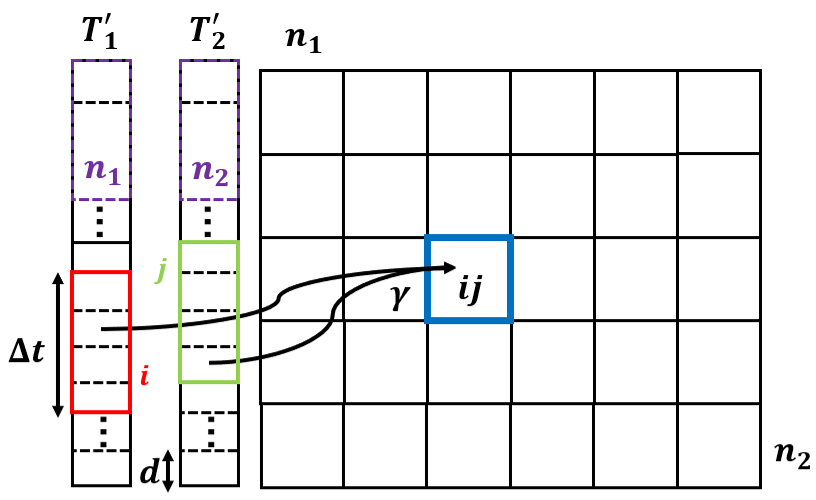
\includegraphics[scale=0.61]{Imagenes/idea.png}
    \caption{Esquema del desplazamiento de una ventana de tiempo sobre las series temporales y el cálculo de la función cross-correlation entre pares de ventanas de tiempo.}
    \label{scan}
\end{figure}

En la figura \ref{scan} se muestra gráficamente la idea detrás cálculo de las funciones de correlación, para una ventana de amplitud $\Delta t$. El tiempo de desplazamiento ($d$) de cada ventana sobre las series temporales, en las $n_{1}$ y $n_{2}$ particiones, permite encontrar los intervalos de tiempo que están más correlacionados. La exactitud de estos intervalos está determinada por el tamaño del desplazamiento. En este trabajo se toma un valor lo suficientemente pequeño en comparación con la duración de las series temporales.

El barrido sobre el lapso de las ventanas de tiempo consiste en calcular la función cross-correlation, como se muestra en la figura \ref{scan}, desde una ventana de amplitud mínima a una de amplitud máxima. Esto genera tantas matrices de correlaciones como amplitudes de ventanas. 

Cabe señalar que los barridos propuestos se realizaron en Python, debido a la facilidad de implementación, manejo y almacenamiento de variables. En el anexo \ref{xcorr_scan_code} se adjunta el código en Python para realizar estas cuentas. Los resultados se almacenan en la variable ${\tt params\char`_time}$ al hacer iterar la función  ${\tt params\char`_xcorr}$ en el ciclo que barre las diferentes ventanas de tiempo.  

Ahora, veamos un ejemplo del cálculo de la función cross-correlation entre un par de ventanas. Tomando $d = 7$ minutos y $\Delta t = 27$ minutos entonces el número de celdas que se obtienen para PSP y SolO son $n_{1} = 15$ y $n_{2} = 31$, respectivamente. En la figura \ref {scan:example1} se muestra la función cross-correlation entre la ventana 10 de la sonda PSP y la ventana 20 de la sonda SolO. El intervalo de tiempo correspondiente en PSP es $04:25 - 04:52$ UT del 27 de septiembre de 2020 y el intervalo de tiempo en SolO es $23:05 - 23:32$ UT del 01 de octubre de 2020. El máximo de correlación es 0.37 y se obtuvo con un desfase de 9.67 minutos entre las series temporales.

\begin{figure}[H]
    \centering
    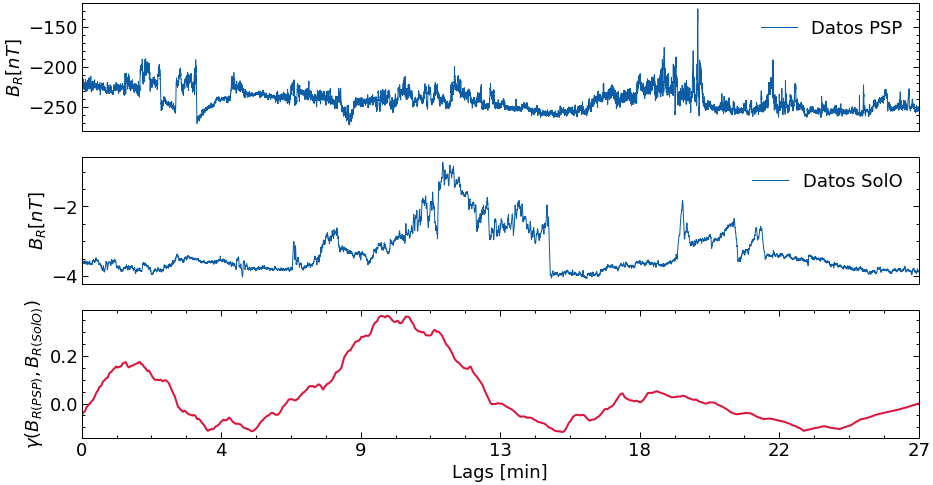
\includegraphics[scale=0.445]{Imagenes/scan_example1.png}
    \caption{Cross-correlation entre los datos de PSP y SolO en una ventana de 27 minutos. De arriba hacia abajo: ventana en PSP, ventana en SolO, función cross-correlation.}
    \label{scan:example1}
\end{figure}

Recordemos que el desfase es el tiempo que se desplazan los datos de una serie temporal respecto de la otra en el cálculo de la función cross-correlation. Aquí reportamos el desfase donde la función de correlación es máxima. Esta magnitud podría contener información física de relevancia, y se debería estudiar sobre aquellos pares de ventanas que presentan la máxima correlación. En nuestro estudio no se ha hecho esto, pero es algo que se podría investigar en un análisis exploratorio futuro. 

Hasta ahora hemos explicado la idea de cómo evaluamos la correlación entre ventanas de dos series. Sin embargo, uno de nuestros objetivos principales es hacer estos cálculos entre las series resultantes de un proceso de filtrado, donde las componentes de alta frecuencia hayan sido eliminadas. Así, primero nos interesa descomponer las series en sus IMFs. Luego se hacen reconstrucciones parciales, al ir disminuyendo las IMFs, hasta quedarnos con un número determinado de aquellas componentes correspondientes a las bajas frecuencias. Y tras cada reconstrucción, calculamos las correlaciones. El número de IMFs que necesitemos considerar, para obtener resultados significativos en el cálculo de las correlaciones, es una de las cosas que queremos determinar en este trabajo.

Este procedimiento se realiza para cada amplitud de ventana. También, como las series pueden descomponer en un número diferente de componentes, en este barrido, la serie con el menor número de IMFs limita las componentes filtradas de la otra serie. Cuando ambas series tienen el mismo número de IMFs entonces el filtro termina con la componente de menor frecuencia más el residuo.       

En la figura \ref {scan:example2} se muestran las reconstrucciones de las ventanas de tiempo de la figura \ref {scan:example1} y su función cross-correlation. Cada reconstrucción se realiza con 5 IMFs. Al reducir las altas frecuencias, los valores de la función de correlación aumentan respecto de la curva de la figura \ref {scan:example1}. El máximo de correlación es 0.42 con un desfase de 9.70 minutos.

\begin{figure}[H]
    \centering
    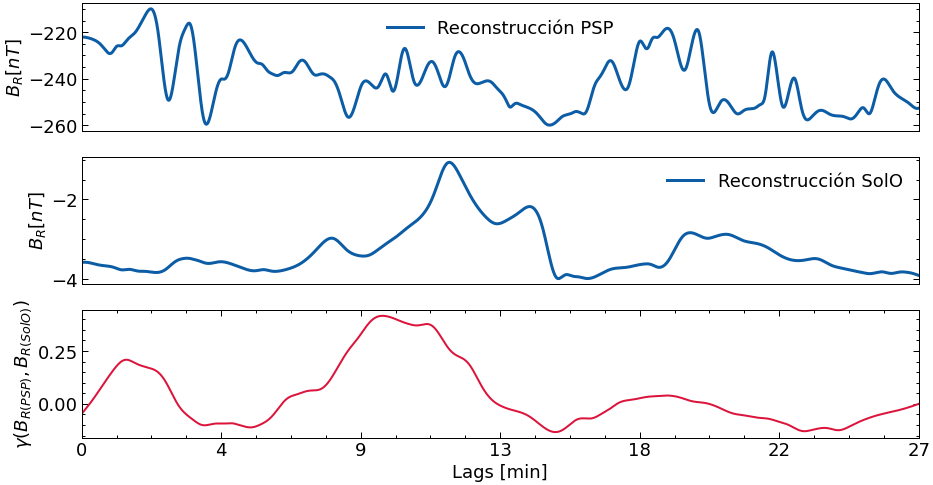
\includegraphics[scale=0.445]{Imagenes/scan_example2.png}
    \caption{Similar a \ref{scan:example1} aunque con los datos (de las ventanas) reconstruidos con las primeras 5 IMFs de baja frecuencia.}
    \label{scan:example2}
\end{figure}

Los cálculos se ejecutaron con las IMFs obtenidas de la implementación del método EMD en Fortran y aquellas resultantes de una implementación en Python \cite{quinn_emd_2021}. Esto se hizo para comparar los resultados obtenidos en Fortran con los de una implementación profesional del EMD. En esta última se fijó el valor límite del criterio de detenimiento del proceso \textit{sifting} en $SD^{*} = 0.3$, como en la implementación de Fortran. 

En nuestro código de Python del anexo \ref{xcorr_scan_code} estas cuentas se muestran para la implementación del EMD de Python. La función ${\tt params\char`_xcorr}$ ejecuta el barrido sobre las IMFs para cada valor de ventana. El residuo y las IMFs extraídas de las series se almacenan en las columnas de un arreglo bidimensional. Las columnas de este arreglo se pueden sumar fácilmente en Python, especificando las columnas a sumar. El arreglo (columna) resultante es la reconstrucción parcial de una serie.

Para cada valor de ventana, todas las posibles correlaciones entre pares de particiones de las series se realizan en un doble ciclo. En cada iteración se calcula el máximo de correlación. Estos valores se ordenan de mayor a menor a través de la función ${\tt get\char`_jixcorrs}$ y se registran en la variable ${\tt max\char`_vals}$. Junto a estos valores se almacenan los índices de las particiones de cada serie. También, para cada máximo de correlación, se evalúa y se almacena el desfase entre cada par de ventanas. De esta manera, el primer valor contiene el máximo de todas las posibles correlaciones y las particiones asociadas. 

Una ligera modificación de la función ${\tt params\char`_xcorr}$ permite efectuar el barrido con los resultados de Fortran. En este caso, las IMFs se introducen externamente como variables globales. Primero, como ya no se utiliza la implementación del EMD en Python, se retiran los parámetros asociados. Luego, se elimina el parámetro de entrada ${\tt field\char`_component}$ así como la lectura de las componentes que se realiza con este parámetro. Finalmente, en esta parte se cargan las IMFs y se limita la duración de las series temporales con los valores de $T'$ correspondientes.

Por último, cabe señalar que las funciones mencionadas son de autoria propia y son las que permiten extraer información del barrido. Dentro de estas funciones se utilizan otras funciones propias de Python para realizar procedimientos de soporte, por ejemplo, la función que permite realizar la descomposición de las series temporales mediante el método EMD. 
     \chapter{Resultados, conclusiones y recomendaciones}

\section{Resultados}

\subsection{Implementación del EMD en Fortran}

\noindent La implementación del método EMD en Fortran se realizó siguiendo el planteamiento de la sección \ref{EMD}. En la figura \ref{fig:emd_comparison} se observa que nuestra implementación genera, en promedio, un mayor número de IMFs respecto de las implementaciones de Python (python 3) y Matlab (versión R2021a), para cualquiera de las series temporales.

\begin{figure}[H]
\centering
\subfigure{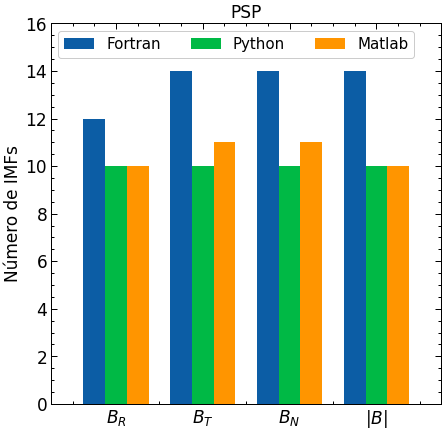
\includegraphics[scale=0.47]{Imagenes/number_imfs_PSP.png}\label{comparison1}}
\subfigure{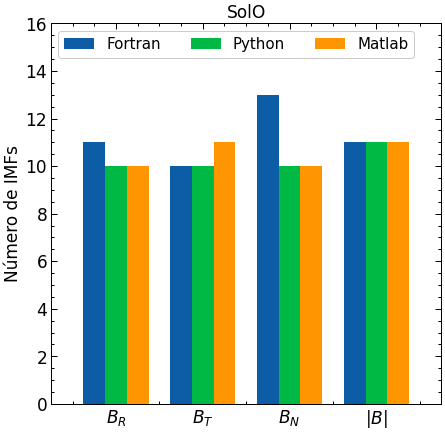
\includegraphics[scale=0.47]{Imagenes/number_imfs_SolO.png}\label{comparison2}}
\caption{Comparación en el número de IMFs resultantes de la descomposición de las series temporales del campo magnético mediante el método EMD en Fortran, Python y Matlab. Izquierda: PSP; derecha: SolO.}
\label{fig:emd_comparison}
\end{figure}

Los resultados dependen de la implementación exacta del método, lo que explica la variabilidad en el número de IMFs entre las diferentes implementaciones. Las principales diferencias pueden deberse al tipo de interpolación para el cálculo de las envolventes, las condiciones de frontera de las envolventes y los criterios de detenimiento del proceso \textit{sifting} o de toda la descomposición, como se vio en la metodología.

\begin{figure}[H]
\centering
\subfigure{\includegraphics[scale=0.36]{imfs_PSP_fortran.png}\label{emdPSP:1}}
\subfigure{\includegraphics[scale=0.36]{imfs_PSP_python.png}\label{emdPSP:2}}
\caption{Resultado de la descomposición de $B_{R}$ de PSP. De arriba hacia abajo: serie temporal de la componente radial del campo magnético; IMFs de la descomposición del método EMD y su residuo. Izquierda: Fortran, 12 IMFs; derecha: Python, 10 IMFs.}
\label{fig:emdPSP}
\end{figure}

Para comparar los resultados de las implementaciones, en la figura \ref{fig:reconstruction_PSP} se muestran las reconstrucciones parciales de la serie temporal $B_{R}$ de PSP, obtenidas mediante las IMFs de Python y Fortran, que se presentan en la figura \ref {fig:emdPSP}. El número de IMFs que utilizan las reconstrucciones de Python y Fortran es $80 \%$ y $75 \%$ del total, respectivamente. Las componentes que no se incluyen son las de mayor frecuencia. Estas reconstrucciones son lo suficientemente buenas pues se parecen a la serie temporal original. La diferencia entre estas reconstrucciones es baja a excepción de puntos con un cambio muy rápido en la señal original. La razón de esto es que las implementaciones difieren un poco al extraer las características locales de las series. Además, notemos que las diferencias entre los resultados de las implementaciones son tan pequeñas, que los valores que cuantifican estas diferencias son uno o dos órdenes de magnitud menores que los valores del campo magnético medidos en las series temporales.

\begin{figure}[H]
    \centering
    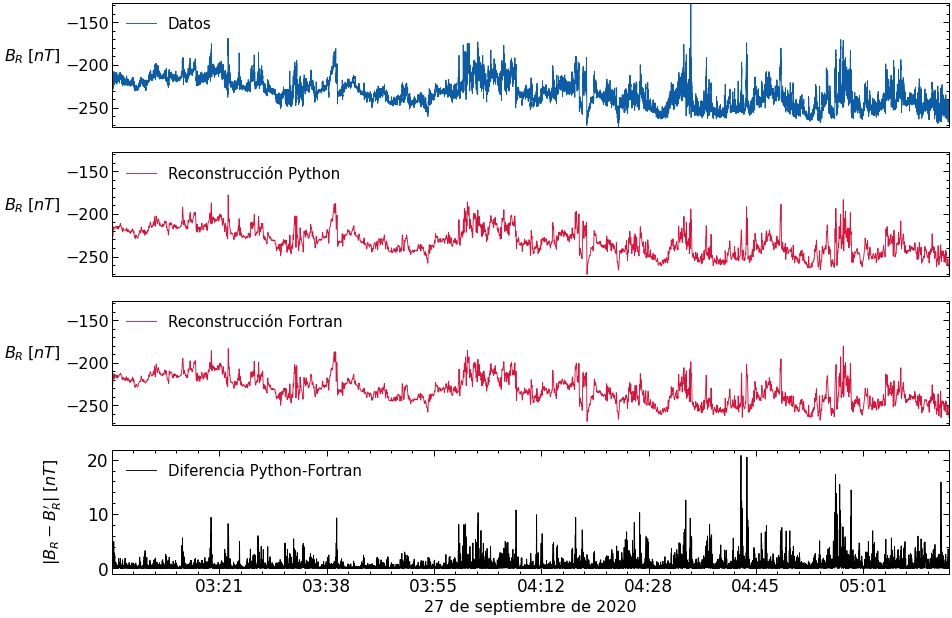
\includegraphics[scale=0.43]{Imagenes/reconstruction_PSP.png}
    \caption{Reconstrucciones de la serie temporal $B_{R}$ de PSP a partir de sus IMFs. De arriba hacia abajo: señal, reconstrucción de Python con $80\%$ IMFs, reconstrucción de Fortran con $75\%$ IMFs, valor absoluto de la diferencia entre las reconstrucciones.}
    \label{fig:reconstruction_PSP}
\end{figure}

\begin{figure}[H]
    \centering
    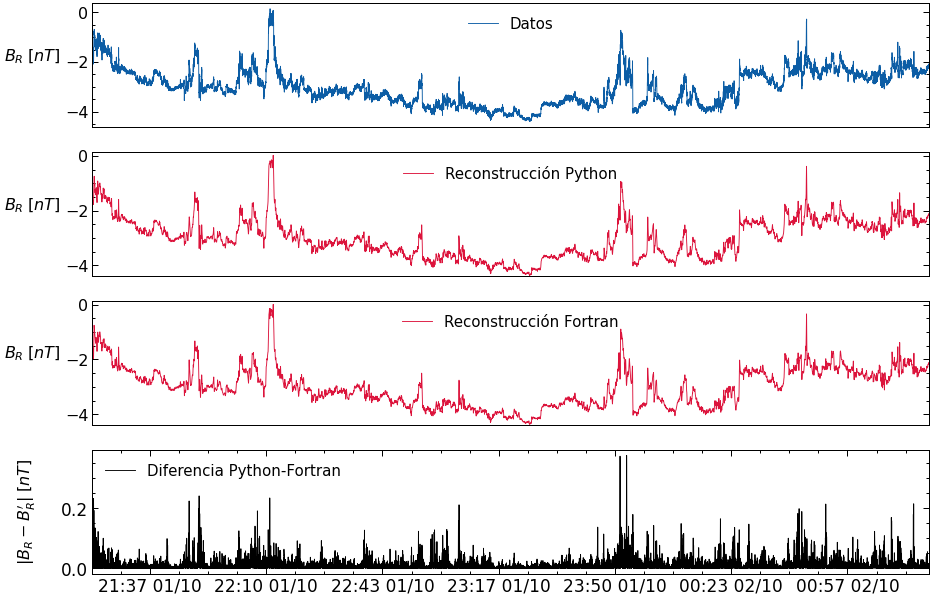
\includegraphics[scale=0.43]{Imagenes/reconstruction_SolO.png}
    \caption{Similar a la figura \ref{fig:reconstruction_PSP} pero para los datos de SolO.}
    \label{fig:reconstruction_SolO}
\end{figure}

Las reconstrucciones de la serie temporal con todas sus IMFs mostraron una diferencia del orden de la precisión de los datos ($\sim 10^{-13}-10^{-14}$). Más aún, los datos originales y las diferentes reconstrucciones con todas las IMFs también dieron estos resultados. Por tanto, a pesar de que las diferentes implementaciones generan un número diferente de IMFs, los resultados entre sí son comparables. Esto valida nuestra implementación realizada en Fortran. 

En la figura \ref{fig:reconstruction_SolO} se muestran las reconstrucciones parciales de la serie temporal $B_{R}$ de SolO, a partir de las IMFs de menor frecuencia en la figura \ref{fig:emdSolO}. Ambas reconstrucciones utilizan $8$ IMFs. En este caso las reconstrucciones parciales se parecen mucho más a la serie temporal original que en los datos de PSP. 

\begin{figure}[H]
\centering
\subfigure{\includegraphics[scale=0.36]{imfs_SolO_fortran.png}\label{emdSolO:1}}
\subfigure{\includegraphics[scale=0.36]{imfs_SolO_python.png}\label{emdSolO:2}}
\caption{Similar a la figura \ref{fig:emdPSP} pero para los datos de SolO. Izquierda: Fortran, 11 IMFs; derecha: Python, 10 IMFs.}
\label{fig:emdSolO}
\end{figure}

\subsection{Correlaciones a baja frecuencia entre ventanas de tiempo de las series temporales}

\noindent En esta sección presentamos los resultados de nuestro análisis exploratorio. Estos resultados se obtuvieron a través de la implementación del método EMD de Python. Resultados similares se obtuvieron con las IMFs calculadas en nuestra implementación de Fortran. 

Debido al poco tiempo disponible para realizar este trabajo, solamente se pudo analizar una de las componentes del campo magnético, y se decidió que fuera la componente radial. Esta componente es predominante en las series temporales estudiadas (en promedio, $B$ y $B_{R}$ son casi paralelas) \cite{telloni_evolution_2021}. Más aún, no todas las componentes son afectadas de la misma manera por la turbulencia del viento solar, pues esta es anisotrópica \cite{duan_anisotropy_2021}. A medida que crece la distancia respecto del Sol, la anisotropía de las fluctuaciones también crece \cite{bruno_effects_1999}, en relación con la evolución de la turbulencia. Sin embargo, las fluctuaciones son mayores en la dirección perpendicular al campo medio que en la dirección paralela \cite{belcher_large-amplitude_1971}. En este caso la componente radial es la menos afectada por la turbulencia. Las razones anteriores hacen que el seguimiento de la componente radial del campo magnético sea más interesante en un primer acercamiento exploratorio, y que el análisis del resto de las componentes vaya más allá del alcance de este estudio.    

El barrido se realizó con ventanas de 10 a 88 minutos en pasos de 2 minutos. El tiempo de desplazamiento ($d$) también fue de 2 minutos. Por otro lado, en el barrido de las IMFs se sumaron hasta 10 componentes de las series temporales, respecto de la implementación del EMD de Python. Esto hizo que el número de operaciones necesarias para el cálculo de las correlaciones en los barridos propuestos fuera superior a $10^4$. Estas operaciones consumieron mucho tiempo computacional y por esta razón se omitieron las ventanas de mayor duración (que son las que tardan más tiempo en computar).    

En la figura \ref{fig3} se muestran los máximos de correlación obtenidos en los barridos de las ventanas de tiempo y las IMFs. Resalta que la tendencia de estos máximos, respecto de todas las ventanas, no varía mucho cuando se consideran más de 5 IMFs en la reconstrucción de las series temporales. Considerar menos de 4 IMFs genera correlaciones altas como consecuencia de una reducción significativa de la información de las series, por la acción del filtrado. 

\begin{figure}
    \centering
    \includegraphics[scale=0.55]{barrido_imfs.png}
    \caption{Máximos de correlación en el barrido sobre la duración de las ventanas de tiempo y el número de IMFs. Entre líneas puntadas se separan tres rangos de ventanas de tiempo para los que se observaron diferentes patrones de correlación relevantes en las series temporales de $B_{R}$.}
    \label{fig3}
\end{figure}

\begin{figure}
\centering
\subfigure[$\Delta t = 20$ minutos]{\includegraphics[scale=0.42]{mapa_corr/fig-20&2.png}\label{fig6: 1}}
\subfigure[$\Delta t = 28$ minutos]{\includegraphics[scale=0.42]{mapa_corr/fig-28&2.png}\label{fig6: 2}}
\subfigure[$\Delta t = 36$ minutos]{\includegraphics[scale=0.42]{mapa_corr/fig-36&2.png}\label{fig6: 3}}
\subfigure[$\Delta t = 44$ minutos]{\includegraphics[scale=0.42]{mapa_corr/fig-44&2.png}\label{fig6: 4}}
\subfigure[$\Delta t = 52$ minutos]{\includegraphics[scale=0.42]{mapa_corr/fig-52&2.png}\label{fig6: 5}}
\subfigure[$\Delta t = 80$ minutos]{\includegraphics[scale=0.42]{mapa_corr/fig-80&2.png}\label{fig6: 6}}
\caption{Mapas de correlaciones para algunas ventanas de tiempo en las series temporales de $B_{R}$ de PSP y SolO. Las correlaciones se calcularon entre datos reconstruidos con 4 IMFs de baja frecuencia. De arriba hacia abajo y de izquierda a derecha: ventanas de tiempo de 20, 28, 36, 44, 52 y 80 minutos.}
\label{fig6}
\end{figure}

Si los valores máximos de una matriz de correlaciones (como la figura \ref{scan}), calculados para una amplitud de ventana, se visualizan en un mapa de calor entonces se pueden observar patrones característicos como los de la figura \ref{fig6}. Estos \textit{mapas de correlaciones} se obtuvieron de las reconstrucciones con las 4 IMFs de menor frecuencia, pues lo observado en la figura \ref{fig3} sugiere que 4 es el número mínimo de IMFs que permiten obtener un buen filtrado de las series y mantener la tendencia de los máximos de correlación, respecto de las series no filtradas. Los valores de la figura \ref{fig3} se corresponden con los máximos de cada uno de los mapas de correlaciones, es decir, aquellos obtenidos en los barridos de las ventanas de tiempo y las IMFs.

Los patrones observados indican que las series temporales contienen varios intervalos de tiempo, de diferente duración, donde su correlación es máxima. En particular, las regiones de mayor correlación para las ventanas entre 22 y 54 minutos fueron relevantes. En este rango de ventanas, los máximos de correlación de la figura \ref{fig3} tienen gradientes pronunciados, disminuyendo rápidamente hasta los 36 minutos y con un pico en los 44 minutos, para después continuar con la tendencia decreciente. Asimismo, podemos notar que alrededor de las ventanas de 22 y 54 minutos existen cambios relativamente grandes en la correlación, para las reconstrucciones con más de 4 IMFs. Además, los intervalos de tiempo que les corresponden a este rango de ventanas se solapan con aquellos que contienen al mismo plasma espacial en las series temporales del campo magnético.   

Las otras ventanas no mostraron mapas de correlaciones con regiones bien definidas y con una diferencia notoria respecto del resto del mapa. Esto lo podemos observar en los paneles \ref{fig6: 1} y \ref{fig6: 6}. Además, para cada IMF, las ventanas menores a 22 minutos presentan máximos de correlación muy altos y casi no varían mucho entre sí, posiblemente debido a que se consideran pocos datos para hacer las cuentas. En el caso de ventanas de más de 54 minutos puede que la semejanza entre las series temporales disminuya y por eso menos intervalos de tiempo muestran alta correlación. En las ventanas de más de 80 minutos se observa un incremento en el máximo de la correlación, aunque los mapas de correlación muestran una única región poco localizada, es decir, valores altos muy dispersos. Esto simplemente reduce los posibles intervalos de tiempo que se pueden relacionar con la presencia del mismo plasma.    

Las tres bandas de ventanas sombreadas de la figura \ref{fig3} se relacionan con las regiones de correlación relevantes de la figura \ref{fig6}. Sólo las bandas donde la correlación disminuye muestran dos regiones localizadas. La banda central es algo así como una transición entre las regiones de las otras bandas. A pesar de la alta correlación de las regiones observadas, no es la alta correlación lo relevante en este estudio. Los cambios significativos en la correlación a medida que se añaden más IMFs son de interés. Quizá las ventanas donde existe un gran salto en la correlación, ya sea para un número determinado de IMFs o al variar las IMFs, podrían ser físicamente significativas. Por ejemplo, en la figura \ref{fig3}, las reconstrucciones con 4 IMFs destacan estos saltos para las ventanas de $22$ y $54$ minutos.

Los expertos suelen utilizan series temporales cuya duración es superior a los $60$ minutos para sus estudios \cite{telloni_evolution_2021}. La razón de esto es que para tiempos de menor duración la turbulencia tiende a destruir las estructuras de menor tamaño o provoca que la correlación entre estas (estructuras) disminuya mucho durante la expansión del viento solar \cite{bruno_turbulence_2016}. Sin embargo, los tiempos encontrados ($\sim 22 - 54$ minutos), con este análisis de carácter puramente exploratorio, podrían tener alguna relevancia física, más allá de la relación con los intervalos de tiempo que contienen al mismo plasma espacial, y por tanto se deberían estudiar más detenidamente para descubrir su importancia.

\begin{figure}
    \centering
    \includegraphics[scale=0.52]{barrido_ventanas_celdas.png}
    \caption{Máximos de correlación respecto del número de IMFs de menor frecuencia que reconstruyen las ventanas de tiempo de las series temporales de $B_{R}$. Las ventanas de 44 y 54 minutos se indican con marcadores diferentes como ejemplo de la tendencia.}
    \label{fig4}
\end{figure}    

En las figuras \ref{fig4} y \ref{fig5} se muestran resultados similares a lo observado en la figura \ref{fig3}. El máximo de correlación no varía mucho para las reconstrucciones con más de 5 IMFs. Además, en la figura \ref{fig4} se observa que el máximo de correlación en cada uno de los mapas se incrementa al reducir el número de IMFs de las señales y que disminuye al considerar ventanas más grandes. Por otro lado, la figura \ref{fig5} indica que los intervalos de tiempo más correlacionados, con 10 IMFs (cuando no se han filtrado las altas frecuencias), no siempre incrementan su correlación al reducir el número de IMFs en la reconstrucción de las señales.          

La reconstrucción de las series temporales de $B_{R}$ con $5$ IMFs mostró una frecuencia característica (frecuencia en el valor máximo del espectro de potencias de Fourier justo antes del comportamiento de ley de potencia en la curva $log-log$; el lector puede dirigirse a las referencias para más detalles, en particular \cite{carbone_arbitrary-order_2018}) de $9\times 10^{-3} Hz$ para PSP y  $1.66\times 10^{-3} Hz$ para SolO. Estos valores son cercanos a la frecuencia característica de la quinta IMF de menor frecuencia, $1\times 10^{-2} Hz$ para PSP y $4.16\times 10^{-3} Hz$ para SolO, lo cual es esperado por la acción del filtro. Estos valores de frecuencia podrían sugerir una escala característica para identificar cuándo las partes no turbulentas de dos series temporales del campo magnético del viento solar están altamente correlacionadas y quizá verificar si pertenecen al mismo plasma. Sin embargo, mayores detalles sobre las implicaciones físicas no son del todo claros y se necesita un mayor estudio.

\begin{figure}
    \centering
    \includegraphics[scale=0.52]{barrido_ventanas_celda_serie.png}
    \caption{Similar a \ref{fig4} pero para las particiones de mayor correlación que se obtienen con la serie temporal completa, es decir, las particiones son fijas en el barrido.}
    \label{fig5}
\end{figure}

\begin{figure}
    \centering
    \includegraphics[scale=0.45]{reconstruccion_54min_0&30.png}
    \caption{Reconstrucción de las series temporales de $B_{R}$ con las 4 IMFs de menor frecuencia en una ventana de 54 minutos. Arriba: datos de PSP en el intervalo de tiempo 03:15-04:09 UT el 27 de septiembre de 2020; abajo: datos de SolO en el intervalo de tiempo 22:20-23:14 UT el 01 de octubre de 2020.}
    \label{fig7}
\end{figure}

\begin{figure}
    \centering
    \includegraphics[scale=0.45]{reconstruccion_54min_23&18.png}
    \caption{Similar a \ref{fig7}. Arriba: datos de PSP en el intervalo de tiempo 04:01-04:55 UT el 27 de septiembre de 2020; abajo: datos de SolO en el intervalo de tiempo 21:56-22:50 UT el 01 de octubre de 2020.}
    \label{fig8}
\end{figure}

En las figuras \ref{fig7} y \ref{fig8} se presenta el caso particular de la reconstrucción de las series temporales (de PSP y SolO) con 4 IMFs de baja frecuencia, para dos ventanas de tiempo de 54 minutos. Se observa que las reconstrucciones se ajustan suavemente al comportamiento de los datos. El valor máximo de la función cross-correlation entre las señales reconstruidas es de $0.705$ para la figura \ref{fig7} y $0.656$ para la figura \ref{fig8}. Los intervalos de tiempo están relacionados con cada una de las regiones relevantes en los mapas de correlación, teniendo los pares de ventanas más correlacionados para 54 minutos. Estos intervalos son entre las horas 03:15 - 04:09 UT del 27 de septiembre de 2020 en PSP y 22:20 - 23:14 UT del 1 de octubre de 2020 en SolO.  Por otro lado, los intervalos de tiempo de las otras reconstrucciones son entre las horas 04:01 - 04:55 UT en PSP y 21:56 - 22:50 UT en SolO, en los días respectivos.  

Las series temporales analizadas en este trabajo se corresponden con los intervalos de tiempo ampliados que se estudiaron en la investigación que se toma de referencia \cite{telloni_evolution_2021}. En otras palabras, no se asegura que toda la duración de las señales pertenece al mismo plasma espacial, sino solamente una parte. Los intervalos de tiempo encontrados, en las regiones de alta correlación, están contenidos o se solapan con aquellos hallados en el estudio anterior, indicando nuevamente que los intervalos reportados son los que contienen la información del mismo plasma espacial.

\section{Conclusiones y recomendaciones}

\noindent Nuestra implementación del método EMD en Fortran produjo, en promedio, un mayor número de IMFs respecto de las implementaciones profesionales en Matlab y Python. Esta diferencia se debe al grado de optimización de las implementaciones. Sin embargo, los resultados fueron comparables dado que la reconstrucción de las series temporales fue similar. Esto permitió validar la implementación hecha en Fortran. 

El cálculo de las correlaciones propuestas se limitó a la componente radial del campo magnético. En el barrido sobre el número de IMFs se estimó que alrededor de 5 IMFs, con la implementación de Python, permiten reconstruir las series de forma adecuada, realizar un buen filtrado de las altas frecuencias y mantener la tendencia de los máximos de correlación para las distintas amplitudes de ventana, con respecto a las series no filtradas.     

Por otro lado, el barrido de las ventanas de tiempo mostró que ventanas entre 22 y 54 minutos presentan una alta correlación (\ref{fig6}) y que sus valores máximos tienen gradientes pronunciados (\ref{fig3}), que los diferencian de ventanas menores a 22 minutos o mayores a 54 minutos. Esto sugiere que las amplitudes de ventana entre 22 y 54 minutos podrían ser físicamente significativas. Sin embargo, este estudio, que tiene un carácter puramente exploratorio, sólo permitió identificar estas amplitudes, pero no se pudo concluir nada sobre sus implicaciones físicas pues los detalles no son del todo claros. Por último, los intervalos de tiempo, asociados a estas amplitudes de ventana, se solapan con aquellos reportados en el estudio anterior \cite{telloni_evolution_2021} sobre los datos analizados en este trabajo, es decir, se relacionan con la información del mismo plasma a distintas distancias.

Finalmente, se recomienda estudiar las propiedades físicas, de la parte no turbulenta de las series temporales, de las ventanas de tiempo entre 22 y 54 minutos para su determinar su relevancia y sus posibles implicaciones físicas. También, un trabajo que siguiera la línea iniciada en este estudio debería investigar las frecuencias características de las reconstrucciones de las series con 5 IMFs y buscar si existe algún significado físico. De igual manera, se debe continuar explorando sobre las otras componentes del campo magnético y revisar el número de IMFs para obtener un buen filtro de las altas frecuencias. 

     
     % Anexos
     \appendix
     \chapter{Anexos}

\section{Código en Fortran con el método EMD}\label{EMD_code}

\begin{spacing}{1.}
\begin{lstlisting}
!============================================================================
!Module containing subroutines to perform the emd algorithm
!============================================================================
module emd_mod
  implicit none
  integer, parameter :: dp = selected_real_kind(15, 307)
  contains
!----------------------------------------------------------------------------
!Adds an element to an array
!----------------------------------------------------------------------------
  subroutine append(array, element)
    integer :: i, insize
    real(dp), intent(in) :: element
    real(dp), dimension(:), allocatable, intent(inout) :: array
    real(dp), dimension(:), allocatable :: outlist

    if(allocated(array)) then
      insize = size(array)
      allocate(outlist(insize+1))
      do i=1,insize          
        outlist(i) = array(i)
      end do
      outlist(insize+1) = element
      deallocate(array)
      call move_alloc(outlist, array) 
    else
      allocate(array(1))
      array(1) = element
    end if
  end subroutine append
!----------------------------------------------------------------------------
!Finds the local maxima and minima of an array and its positions in x-axis 
!----------------------------------------------------------------------------
  subroutine findLocalMaximaMinima(x, array, x_minima, minima, x_maxima, maxima)
    integer :: N, i, m, num_minima, num_maxima
    real(dp), intent(in) :: x(:), array(:)
    real(dp), dimension(:), intent(inout), allocatable :: x_minima, minima, &
       x_maxima, maxima
    real(dp), dimension(:), allocatable :: x_aux, y_aux 

    allocate(x_minima(0), minima(0), x_maxima(0), maxima(0))
    N = size(array)
    num_minima = 0
    num_maxima = 0
    do i=2, N-1
      !condition for local minima
      if((array(i-1)>array(i)).and.(array(i)<array(i+1))) then 
        call append(x_minima, x(i))
        call append(minima, array(i))
        num_minima = num_minima + 1
      !condition for local maxima
      else if((array(i-1)<array(i)).and.(array(i)>array(i+1))) then 
        call append(x_maxima, x(i))
        call append(maxima, array(i))
        num_maxima = num_maxima + 1
      end if
    end do
    
    !Boundary conditions to perform Cubic Splines
    !This adds 2 values to local maxima and minima: 4 in total
    !To get the exact number, the size of each must be reduced by  2
    if((num_minima .ne. 0).and.(num_maxima .ne. 0)) then
    !boundary conditions for minima
      m = size(x_minima)
      allocate(x_aux(m+2), y_aux(m+2))
      x_aux(1) = x(1)
      x_aux(2:m+1) = x_minima(1:m)
      x_aux(m+2) = x(N)
      y_aux(1) = minima(1)
      y_aux(2:m+1) = minima(1:m)
      y_aux(m+2) = minima(m)
      deallocate(x_minima, minima)
      allocate(x_minima(m+2), minima(m+2))
      x_minima = x_aux
      minima = y_aux 
      deallocate(x_aux, y_aux)

    !boundary conditions for maxima
      m = size(x_maxima)
      allocate(x_aux(m+2), y_aux(m+2))
      x_aux(1) = x(1)
      x_aux(2:m+1) = x_maxima(1:m)
      x_aux(m+2) = x(N)
      y_aux(1) = maxima(1)
      y_aux(2:m+1) = maxima(1:m)
      y_aux(m+2) = maxima(m)
      deallocate(x_maxima, maxima)
      allocate(x_maxima(m+2), maxima(m+2))
      x_maxima = x_aux
      maxima = y_aux 
      deallocate(x_aux, y_aux)
    end if
  end subroutine
!----------------------------------------------------------------------------
!Performs Cubic Splines using 'x', 'y' and 'x_splines' vectors as input and 
!returns 'y_splines' vector as output, interpolating the data in 'y'  
!----------------------------------------------------------------------------
  subroutine cubic_splines(x, y, x_splines, y_splines)
    real(dp), dimension(:), intent(in) :: x, y, x_splines
    real(dp), dimension(:), intent(inout) :: y_splines
    real(dp), dimension(:), allocatable :: b, h, c, d, l, dd, u
    integer :: i, j, k, Nnodes, N_splines
    real(dp) :: xinter, yinter

    Nnodes = size(x)
    N_splines = size(x_splines)
    allocate(b(Nnodes),h(Nnodes-1),c(Nnodes-1),d(Nnodes-1),l(Nnodes), &
      dd(Nnodes),u(Nnodes)) 

    !Tridiagonal matrix and vector of coefficients for the method
    !A(l, dd, u)x = b   
    do i = 1, Nnodes-1
      h(i) = x(i+1)-x(i)
      l(i+1) = 1.0_dp/h(i)
      u(i) = 1.0_dp/h(i)
      if(i>1) then 
        dd(i) = 1./h(i-1) + 1.0_dp/h(i)
        b(i) = y(i+1)/(h(i)*h(i)) + y(i)*(1./(h(i-1)*h(i-1))-1./(h(i)*h(i))) - &
          y(i-1)/(h(i-1)*h(i-1))
      end if
    end do !i
    dd(1) = 1.0_dp/h(1)
    dd(Nnodes) = 1.0_dp/h(Nnodes-1)
    dd(1:Nnodes) = 2.0_dp*dd(1:Nnodes)
    b(1) = (y(2)-y(1))/(h(1)*h(1))
    b(Nnodes) = (y(Nnodes)-y(Nnodes-1))/(h(Nnodes-1)*h(Nnodes-1))
    b(1:Nnodes) = 3.0_dp*b(1:Nnodes)

    !Solution of the linear system
    do i=2,Nnodes
      l(i) = l(i)/dd(i-1)
      dd(i) = dd(i) - l(i)*u(i-1)
      b(i) = b(i)-l(i)*b(i-1)
    end do !i
    b(Nnodes) = b(Nnodes)/dd(Nnodes)
    do i = Nnodes-1, 1, -1
      b(i) = (b(i) - u(i)*b(i+1))/dd(i)
    end do !i

    !Cubic Splines Interpolation
    do i = 1, Nnodes-1
      c(i) = 3.0_dp*(y(i+1)-y(i))/(h(i)*h(i))-2.0_dp*b(i)/h(i)-b(i+1)/h(i)
      d(i) = 2.0_dp*(y(i)-y(i+1))/(h(i)**3) + (b(i)+b(i+1))/(h(i)*h(i))
    end do 
    j = 1
    do i = 1, N_splines
      xinter = x_splines(i)
      do k = 1, Nnodes-1
        if((x(k)<xinter).and.(xinter < x(k+1))) j = k
      end do !k
      yinter = y(j) + b(j)*(xinter-x(j)) + c(j)*(xinter-x(j))*(xinter-x(j)) + &
        d(j)*(xinter-x(j))**3 
      y_splines(i) = yinter
    end do !i
    deallocate(h,b,c,d,l,dd,u)  
  end subroutine
!----------------------------------------------------------------------------
!Performs the main steps in the sifting process.
!It takes 'x' and 'y' as input vectors and returns a proto-IMF 'hk' and also
!'mean' and 'diff_extremas_zeros' in order to check if 'hk' is an IMF.
!----------------------------------------------------------------------------
  subroutine sifting_steps(x, y, hk, mean, diff_extremas_zeros)
    real(dp), dimension(:), intent(in) :: x, y
    real(dp), dimension(:), intent(inout) :: hk
    real(dp), dimension(:), allocatable :: x_minima, minima, x_maxima, maxima, &
      ys_low, ys_up, ys_mean
    integer, intent(inout) :: diff_extremas_zeros
    real(dp), intent(inout) :: mean
    integer :: N_file, i, number_zero_crossings

    N_file = size(x) 
    call findLocalMaximaMinima(x, y, x_minima, minima, x_maxima, maxima) 
    allocate(ys_low(N_file))
    call cubic_splines(x_minima, minima, x, ys_low)
    allocate(ys_up(N_file))
    call cubic_splines(x_maxima, maxima, x, ys_up)
    allocate(ys_mean(N_file))
    ys_mean = 0.5*(ys_low + ys_up)

    hk = y - ys_mean
    mean = 0.0_dp
    do i = 1, N_file
      mean = mean + hk(i)
    end do
    mean = mean/N_file

    number_zero_crossings = 0
    do i = 1, N_file - 1
      if(hk(i)*hk(i+1) < 0) number_zero_crossings = number_zero_crossings + 1
    end do

    diff_extremas_zeros = abs(size(maxima)+size(minima)-number_zero_crossings - 4)
    !We subtract 4 to correct the size of maxima and minima
    deallocate(x_minima, minima, x_maxima, maxima, ys_low, ys_up, ys_mean)
  end subroutine
!----------------------------------------------------------------------------
!Standard Deviation criterion to stop the sifting process
!----------------------------------------------------------------------------
  subroutine stopping_criterion1(hkm1, hk, SD)
    real(dp), dimension(:), intent(in) :: hkm1, hk
    real(dp), intent(inout) :: SD
    integer :: i, total_time
    real(dp), parameter :: eps=1e-8

    total_time = size(hk)
    SD = 0.0_dp
    do  i = 1, total_time
        SD = SD + abs(hk(i)-hkm1(i))*abs(hk(i)-hkm1(i))/(hkm1(i)*hkm1(i)+eps)
    end do
  end subroutine
!----------------------------------------------------------------------------
!Evaluates if the input parameters guarantee an IMF
!----------------------------------------------------------------------------
  subroutine is_imf(param1, param2, success_imf)
    !Difference between the number of extremas and zero crossings
    integer, intent(in) :: param1 
    real(dp), intent(in) :: param2 !mean of Proto-IMFs
    logical, intent(inout) :: success_imf
    real(dp), parameter :: eps_mean = 4e-2 !chosen mean tolerance

    if((param1 <= 1) .and. (abs(param2) <= eps_mean)) then 
      success_imf = .true.
    else
      success_imf = .false.
    end if
  end subroutine
!----------------------------------------------------------------------------
!Evaluates the number of extremas of the residue to stop the decomposition
!----------------------------------------------------------------------------
  subroutine residual_condition(x, r, num_residual_extremas)
    real(dp), dimension(:), intent(in) :: x, r
    integer, intent(inout) :: num_residual_extremas
    real(dp), dimension(:), allocatable :: rx_minima, r_minima, rx_maxima, r_maxima
    integer :: size_minima, size_maxima

    !Precision correction in the residual values. 
    !This avoids getting wrong IMFs.
    call findLocalMaximaMinima(x, anint(r*1e8)/1e8, rx_minima, r_minima, & 
      rx_maxima, r_maxima)
    size_minima = size(r_minima)
    size_maxima = size(r_maxima)
    !Size correction for minima and maxima
    if((size_minima.ne.0).and.(size_maxima.ne.0)) then 
      num_residual_extremas = size_minima + size_maxima - 4
    else
      num_residual_extremas = 0
    end if
    deallocate(rx_minima, r_minima, rx_maxima, r_maxima)
  end subroutine 
end module
!============================================================================
!Main program to perform EMD method on magnetic time series.
!============================================================================
program emd
  use emd_mod
  implicit none

  !MAX_IMFs~log2(N): in this case MAX_IMFs~ 16, 17: expected number of IMFs
  !MAX_PMFs: maximum number of iterations to perform the sifting process
  integer, parameter :: MAX_IMFs=16 + 2, MAX_PMFs=20
  real, parameter :: SD_threshold = 0.3_dp
  integer :: io1=1, io2=2
  integer :: N_file
  real(dp), dimension(:), allocatable :: x, y, hkm1, hk, rj, & 
    time, Br, Bn, Bt, B
  integer :: i, diff_extremas_zeros, num_residual_extremas, num_IMFs, it_sift
  character (len=80) :: nfout
  real(dp) :: mean, SD
  logical :: success_imf

  !size of time series data, name of output file with IMFs
  N_file = 62400 !PSP
  nfout = 'imfs_PSP_Br.dat'  
  !N_file = 115201 !SolO
  !nfout = 'imfs_SolO_B.dat'    
  nfout = trim(nfout)

  allocate(x(N_file), y(N_file), hk(N_file), hkm1(N_file), rj(N_file), &
    time(N_file), Br(N_file), Bt(N_file), Bn(N_file), B(N_file))

  !data reading
  open(unit=io1, file='pspr_20200927_0305_20200927_0515.txt', action='read')
  !open(unit=io1, file='solo_20201001_2120_20201002_0120.txt', action='read')
  do i = 1, N_file
    read(io1, *) time(i), Br(i), Bt(i), Bn(i), B(i)
  end do 
  close(io1)

  !variables on which the EMD method will be applied
  x(1:N_file) = time(1:N_file)/8.0_dp !sample rate = 8Hz
  y(1:N_file) = Br(1:N_file)

  open(unit=io2, file=nfout, status='unknown', action='write')
  
  !Residual condition: monotonous or constant behavior: at most 1 extrema
  num_residual_extremas = 2
  num_IMFs = 0
  rj = y !initial condition for residue
!---------------------------------EMD---------------------------------------
  do while((num_residual_extremas>1).and.(num_IMFs<MAX_IMFs))
    num_IMFs = num_IMFs + 1
    print*, 'IMF: ', num_IMFs
    hkm1 = rj

    !------------------------SIFTING----------------------------------------
    SD = 1.0_dp
    it_sift = 0
    do while((SD>SD_threshold).and.(it_sift<MAX_PMFs))
      it_sift = it_sift + 1
      hk = 0.0_dp
      call sifting_steps(x, hkm1, hk, mean, diff_extremas_zeros)
      call is_imf(diff_extremas_zeros, mean, success_imf)
      call stopping_criterion1(hkm1, hk, SD)
      !condition to stop sifting
      if(success_imf.eqv.(.true.)) exit
      hkm1 = hk
    end do !end of sifting process
    
    !report of sifting results 
    write(*, "(A5, I2, A10, I5, A8, E20.8, A7, L1, A12, F20.8)") &
      '#it: ', it_sift, '| param1: ', diff_extremas_zeros, &
        '| mean: ', mean, '| imf: ', success_imf, '| criterion: ', SD

    if(it_sift==MAX_PMFs) then 
      print*, 'Approximated sifting'
    else if (SD<0.3_dp) then 
      print*, 'SD condition achieved'
    end if

    !residue update
    rj = rj - hk
    write(io2, *) hk
    call residual_condition(x, rj, num_residual_extremas)
    print*, '|---------Extrema of residue---------|', num_residual_extremas
  end do !end of EMD

  write(io2, *) rj

  print*, 'Extrema of residue: ', num_residual_extremas
  print*, 'Number of IMFS: ', num_IMFs

  deallocate(x, y, hkm1, hk, rj, time, Br, Bn, Bt, B)
  close(io2)
end program
!============================================================================
\end{lstlisting}
\end{spacing}

\section{Código en Python para realizar el barrido sobre las ventanas de tiempo y el número de IMFs}\label{xcorr_scan_code}

\begin{spacing}{1.}
\begin{minted}{python}
#=============================================================================
#Program to perform the cross-correlation scan on the time windows and on 
#the number of IMFS
#=============================================================================
#libraries
import numpy as np
import emd as emd2
import numba
from numba import jit
import seaborn as sns; sns.set_theme()

#data
psp_data = np.loadtxt('pspr_20200927_0305_20200927_0515.txt')
psp_data = np.transpose(psp_data)
psp_data[0] = psp_data[0]/8.
solo_data = np.loadtxt('solo_20201001_2120_20201002_0120.txt')
solo_data = np.transpose(solo_data)
solo_data[0] = solo_data[0]/8.
#-----------------------------------------------------------------------------
#Functions
#-----------------------------------------------------------------------------
#Cross-Correlation function
@numba.jit
def cross_corr(x, y):
  n = len(x)
  mean_x = np.mean(x)
  mean_y = np.mean(y)
  std_x = np.std(x)
  std_y = np.std(y)

  xcorr = []
  for k in range(n):
    suma = 0.
    for i in range(n-k):
      suma += (x[i]-mean_x)*(y[i+k]-mean_y)
    xcorr.append(suma)
  xcorr = np.array(xcorr)/(n*std_x*std_y)
  return xcorr

#Function to get the partitions of PSP and SolO (portion of the signals) 
#of the correlation values from the maximum to the minimum
def get_jixcorrs(W):
  length = np.size(W)
  aux = np.reshape(W, (1, length))
  aux2 = np.sort(aux, kind='quicksort')
  aux3 = [np.where(W == aux2[0][i]) for i in range(length)]
  indexs = []
  for k in range(length):
    i, = aux3[k][1]
    j, = aux3[k][0]
    indexs.append([j, i, W[j][i]])
  indexs = indexs[::-1]
  return indexs
#Funtion to perform the cross-correlation scan on the number of IMFS
def params_xcorr(field_component, time_min, delay_min):
  #EMD parameters
  config = emd2.sift.get_config('sift')
  config['imf_opts/sd_thresh'] = 0.3

  #parameters
  T1 = 62400 #130 min PSP
  T2 = 115201 #240 min SolO
  time_width = time_min*60*8
  delay = delay_min*60*8 #time to change from one partition to another 
  n_inter1 = int(np.floor((T1-time_width)/delay)) + 1
  n_inter2 = int(np.floor((T2-time_width)/delay)) + 1
  Tp1 = time_width + delay*(n_inter1-1) #<=T1
  Tp2 = time_width + delay*(n_inter2-1) #<=T2

  #data
  x1 = psp_data[field_component][:Tp1]
  x2 = solo_data[field_component][:Tp2]
  
  #EMD
  imf1 = emd2.sift.sift(x1) #Residue included
  imf2 = emd2.sift.sift(x2)
  num_imfs1 = imf1.shape[1]-1
  num_imfs2 = imf2.shape[1]-1
  start_index_imfs1 = [i for i in range(num_imfs1)]
  start_index_imfs2 = [i for i in range(num_imfs2)]

  #SCAN
  params = []
  print('Time window: {} minutes'.format(time_min))
  sum_imfs = min(start_index_imfs1[-1], start_index_imfs2[-1])
  for k in range(sum_imfs):
    print('# imfs added : PSP({}), SolO({})'.format(num_imfs1-k, num_imfs2-k))

    #Elimination of high frequencies
    y1 = np.sum(imf1[:, start_index_imfs1[k] : ], axis=1)
    y2 = np.sum(imf2[:, start_index_imfs2[k] : ], axis=1)

    #cross-correlation between partitions over the time series
    #scan for a particular time window
    xcorrs = []
    max_lags = []
    for i in range(n_inter1):
      start1 = i*delay
      end1 = time_width + i*delay
      for j in range(n_inter2):
        start2 = j*delay
        end2 = time_width + j*delay
        aux = cross_corr(y1[start1:end1], y2[start2:end2])
        index, = np.where(aux == np.max(aux))
        xcorrs.append(np.max(aux))
        max_lags.append(index[0])

    xcorr_map = np.reshape(xcorrs, (n_inter1, n_inter2))
    xcorr_lags = np.reshape(max_lags, (n_inter1, n_inter2))
    max_vals = get_jixcorrs(xcorr_map)

    #map of maximum correlations
    ticks_step = 8
    xlabels0 = np.arange(time_min+1, time_min+delay_min*(n_inter2-1), delay_min, dtype=int)
    ylabels0 = np.arange(time_min+1, time_min+delay_min*(n_inter1-1), delay_min, dtype=int)
    xlabels1 = np.char.mod('%d', xlabels0)
    ylabels1 = np.char.mod('%d', ylabels0)
    xticks = np.arange(0, n_inter2, 1)
    yticks = np.arange(0, n_inter1, 1)

    fig, ax = plt.subplots(figsize=(width, heigth))
    ax = sns.heatmap(xcorr_map, vmin=0, vmax=1, cmap='inferno', 
      cbar_kws={'label': "correlation", 'pad': 0.005}, annot_kws={"size": 17})
    plt.text(0.35, 0.9, "Maximum = {:.3f}".format(np.max(xcorr_map)), fontsize=17,
       transform=plt.gcf().transFigure)
    ax.invert_yaxis()
    ax.set_xlabel(r"$t(SolO) \; [min]$", fontsize=17)
    ax.set_ylabel(r'$t(PSP) \; [min]$', fontsize=17)  

    ax.set_yticks(yticks[1::ticks_step])
    ax.set_yticklabels(ylabels1[::ticks_step])
    ax.set_xticks(xticks[1::ticks_step])
    ax.set_xticklabels(xlabels1[::ticks_step])
    plt.yticks(rotation=0)
    #save map of maximum correlations in img folder
    plt.savefig('img/fig-'+ str(num_imfs1 - start_index_imfs1[k]) + '&' + 
      str(num_imfs2 - start_index_imfs2[k]) + '_' + str(time_min) + '&'+ 
      str(delay_min) + '.png')
    plt.close(fig)
    
    params.append([[time_min, delay_min, num_imfs1 - start_index_imfs1[k], 
      num_imfs2 - start_index_imfs2[k]], max_vals, xcorr_map, xcorr_lags])
  return params

#Numba function test: needed for it to perform better
x1 = psp_data[1]
x2 = solo_data[1]
test = cross_corr(x1, x2)
#-----------------------------------------------------------------------------
#Main part of the program: It performs the cross-correlation scan 
#on the time windows and on the number of IMFS for some time windows.
#-----------------------------------------------------------------------------
time_mins = np.arange(10, 90, 2)
delay_min = 2
params_time = []

for i in time_mins:
    params_time.append(params_xcorr(1, i, delay_min))
#=============================================================================
\end{minted}
\end{spacing}
    
    % Bibliografía
    \renewcommand\bibname{Referencias bibliográficas}
    %\bibliographystyle{plain}
    \addcontentsline{toc}{chapter}{Bibliografía}
    %\pagenumbering{gobble}
    \printbibliography
    %\bibliography{referencias-tic}

\end{document}
